\graphicspath{{images/}}

\section{Vektorgeometrie}

\begin{definition}{Vektor}
    Objekt, das Betrag und Richtung hat.
    \begin{itemize}
        \item $\overrightarrow{0} = $ Nullvektor (Betrag = 0)
        \item $\overrightarrow{e} = $ Einheitsvektor (Betrag = 1)
        \item $-\overrightarrow{a} = $ Gegenvektor von $\overrightarrow{a}$
    \end{itemize}
\end{definition}

\begin{concept}{Einheitsvektor}
    $$\overrightarrow{e_a} = \frac{\overrightarrow{a}}{|\overrightarrow{a}|}$$  
\end{concept}

\begin{definition}{Kollinear (Parallel)}
    Zwei Vektoren sind kollinear, wenn sie auf einer Geraden liegen. Ein Vektor ist ein Vielfaches des anderen.
\end{definition}

\begin{definition}{Komplanar}
    Drei Vektoren sind komplanar, wenn sie in einer Ebene liegen. Die Vektoren sind linear abhängig.
\end{definition}

\begin{definition}{Orthogonal (Senkrecht)}
    Zwei Vektoren sind orthogonal, wenn der Winkel zwischen ihnen 90° beträgt. 
    $$\overrightarrow{a} \cdot \overrightarrow{b} = 0 \rightarrow \text{ orthogonal}$$
\end{definition}

\begin{concept}{Orthogonale Projektion}
    von $\overrightarrow{b}$ auf $\overrightarrow{a}$ $(0 \neq \varphi \neq \frac{\pi}{2})$:
    $$\overrightarrow{b}_{\perp a} = \frac{\overrightarrow{a} \cdot \overrightarrow{b}}{|\overrightarrow{a}|^2} \cdot \overrightarrow{a}, \quad |\overrightarrow{b}_{\perp a}| = \frac{|\overrightarrow{a} \cdot \overrightarrow{b}|}{|\overrightarrow{a}|}$$
\end{concept}

\begin{formula}{Vektoraddition}
    $$\overrightarrow{a} + \overrightarrow{b} = \begin{pmatrix} a_x + b_x\\ a_y + b_y \end{pmatrix}$$
\end{formula}

\begin{formula}{Skalarmultiplikation}
    $$\lambda \cdot \overrightarrow{a} = \begin{pmatrix}
    \lambda \cdot a_x \\
    \lambda \cdot a_y
    \end{pmatrix}$$
\end{formula}

\begin{formula}{Skalarprodukt}
    $$\overrightarrow{a} \cdot \overrightarrow{b} = a_x \cdot b_x + a_y \cdot b_y = |\overrightarrow{a}| \cdot |\overrightarrow{b}| \cdot \cos(\varphi)$$
\end{formula}

\begin{formula}{Gegenvektor}
    $$-\overrightarrow{a} = \begin{pmatrix}
    -a_x \\
    -a_y
    \end{pmatrix}$$
\end{formula}

\begin{formula}{Betrag}
    $$|\overrightarrow{a}| = \sqrt{a_x^2 + a_y^2}$$
\end{formula}

\begin{formula}{Winkelberechnung}
    $$\cos(\varphi) = \frac{\overrightarrow{a} \cdot \overrightarrow{b}}{|\overrightarrow{a}| \cdot |\overrightarrow{b}|} = \frac{a_x b_x + a_y b_y}{\sqrt{a_x^2 + a_y^2} \cdot \sqrt{b_x^2 + b_y^2}  } $$
\end{formula}

\begin{formula}{Vektorprodukt}
    \begin{itemize}
        \item $|\overrightarrow{a} \times \overrightarrow{b}| = |\overrightarrow{a}| \cdot |\overrightarrow{b}| \cdot \sin(\varphi)$
        \item $\overrightarrow{a} \times \overrightarrow{b}$ ist orthogonal zu $\overrightarrow{a}$ und $\overrightarrow{b}$
        \item $\overrightarrow{a} \times \overrightarrow{b} \neq \overrightarrow{b} \times \overrightarrow{a}$
    \end{itemize}
        $$\overrightarrow{a} \times \overrightarrow{b} = \left(\begin{array}{ccc}
        a_y \cdot b_z &-& a_z \cdot b_y \\
        a_z \cdot b_x &-& a_x \cdot b_z \\
        a_x \cdot b_y &-& a_y \cdot b_x
        \end{array}\right)$$
    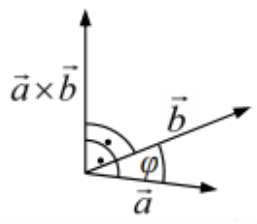
\includegraphics[width=0.2\linewidth]{vektorprodukt.png}
\end{formula}

\begin{formula}{Fläche des aufgespannten Parallelogramms}
    $$h = |\overrightarrow{b}| \cdot \sin(\varphi)$$
    $$A = |\overrightarrow{a} \cdot h = |\overrightarrow{a} \times \overrightarrow{b}| = |\overrightarrow{a}| \cdot |\overrightarrow{b}| \cdot \sin(\varphi)$$
    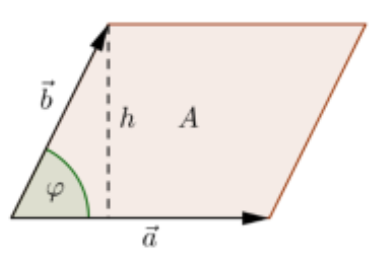
\includegraphics[width=0.3\linewidth]{parallelogramm.png}
\end{formula}

\begin{definition}{Gerade}
    in der Ebene und im Raum
    \begin{itemize}
        \item $\overrightarrow{r}(A) = \overrightarrow{r}(P) + \lambda \cdot \overrightarrow{PQ}$
        \item $g: \overrightarrow{r}(P) + \lambda \cdot \overrightarrow{a}$
    \end{itemize}
    Der Punkt P heisst Aufpunkt, der Richtungsvektor $\overrightarrow{a}  = \overrightarrow{PQ}$ von g.\\
    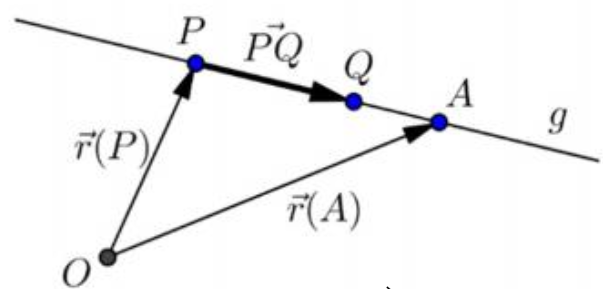
\includegraphics[width=0.3\linewidth]{gerade.png}
\end{definition}

\begin{KR}{Abstand Punkt-Gerade}
    \begin{enumerate}
        \item $\overrightarrow{BA} = \overrightarrow{r}(A) - \overrightarrow{r}(B)$
        \item $0 = \overrightarrow{BA} \cdot \overrightarrow{a}$
        \item Length $= |\overrightarrow{BA}| = \frac{|\overrightarrow{PA} \times \overrightarrow{a}|}{|\overrightarrow{a}|}$
    \end{enumerate}
\end{KR}

\begin{example}
    $$g: \begin{pmatrix} 1 \\ 13 \end{pmatrix} + \lambda \begin{pmatrix} 3 \\ 5 \end{pmatrix}, \quad A(3|-1)$$
    \begin{enumerate}
        \item $\overrightarrow{BA} = \vec{r} \cdot \begin{pmatrix} 3 \\ -1 \end{pmatrix} - \vec{r} \cdot \begin{pmatrix} 1 + 3 \lambda \\ 13 + 5 \lambda \end{pmatrix}$
        \item $0 = \begin{pmatrix} 3 - 1 - 3 \lambda \\ -1 - 13 - 5 \lambda \end{pmatrix} \cdot \begin{pmatrix} 3 \\ 5 \end{pmatrix} \rightarrow \lambda = x$
        \item Length $ = \left| \begin{pmatrix} 2 - 3x \\ -14 - 5x \end{pmatrix} \right|$ 
    \end{enumerate}
    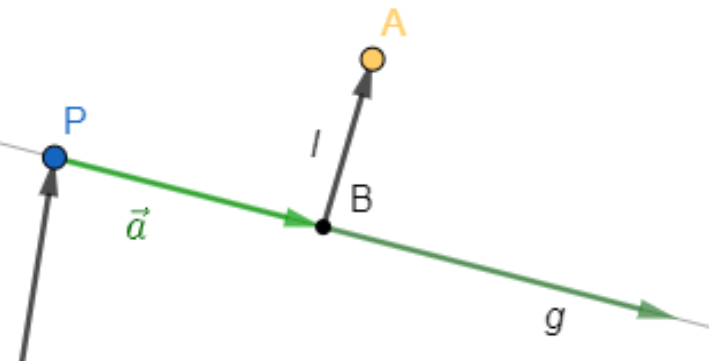
\includegraphics[width=0.3\linewidth]{abstand.png}
\end{example}

\begin{KR}{Abstand Gerade-Gerade}
    \begin{enumerate}
        \item $\overrightarrow{BA} = \overrightarrow{r}(A) - \overrightarrow{r}(B)$
        \item $\overrightarrow{a} \times \overrightarrow{b} = \overrightarrow{n}$
        \item Length $= \frac{|\overrightarrow{BA} \cdot \overrightarrow{n}|}{|\overrightarrow{n}|}$
    \end{enumerate}
\end{KR}

\begin{KR}{Abstand Punkt-Ebene}
    \begin{enumerate}
        \item $\overrightarrow{BA} = \overrightarrow{r}(A) - \overrightarrow{r}(B)$
        \item $0 = \overrightarrow{BA} \cdot \overrightarrow{n}$
        \item Length $= |\overrightarrow{BA}| = \frac{|\overrightarrow{PA} \cdot \overrightarrow{n}|}{|\overrightarrow{n}|}$
    \end{enumerate}
\end{KR}

\begin{definition}{Ebene}
    kann durch 3 Punkte festgelegt werden
    \begin{itemize}
        \item Die Vektoren $\overrightarrow{PA}$, $\overrightarrow{PR}$, $\overrightarrow{PQ}$ sind komplanar
        \item $\overrightarrow{PA} = \lambda \cdot \overrightarrow{PR} + \mu \cdot \overrightarrow{PQ}$
    \end{itemize}
    $$\overrightarrow{r}(A) = \overrightarrow{r}(P) + \lambda \cdot \overrightarrow{PR} + \mu \cdot \overrightarrow{PQ}$$
    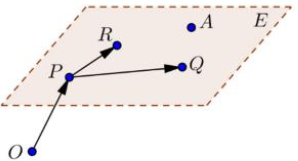
\includegraphics[width=0.3\linewidth]{ebene.png}
\end{definition}

\begin{concept}{Parameterdarstellung} der Ebene
    $$E: \overrightarrow{r}(P) + \lambda \cdot \overrightarrow{a} + \mu \cdot \overrightarrow{b}$$
    $$E: \overrightarrow{n} = \overrightarrow{a} \times \overrightarrow{b}$$
\end{concept}
    
\begin{example}
    $$E: 2x + 7y - 4z + 1 = 0$$
    Punkte einsetzen: $(0|0|z), (1|0|z), (0|1|z)$
    \vspace*{2mm}
    \begin{itemize}
        \item $2 \cdot 0 + 7 \cdot 0 - 4 \cdot z + 1 = 0 \Rightarrow z = \frac{1}{4}$
        \item $2 \cdot 1 + 7 \cdot 0 - 4 \cdot z + 1 = 0 \Rightarrow z = \frac{3}{4}$
        \item $2 \cdot 0 + 7 \cdot 1 - 4 \cdot z + 1 = 0 \Rightarrow z = \frac{8}{4}$
    \end{itemize}
    \vspace*{2mm}
    $$E: \begin{pmatrix} 0 \\ 0 \\ \frac{1}{4} \end{pmatrix} +
    \lambda \begin{pmatrix} 1 \\ 0 \\ \frac{2}{4} \end{pmatrix} +
    \mu \begin{pmatrix} 0 \\ 1 \\ \frac{7}{4} \end{pmatrix}$$
\end{example}

\begin{concept}{Koordinatendarstellung} der Ebene
    $$E: ax + by + cz + d = 0$$
    $$\vec{n} = \begin{pmatrix} a \\ b \\ c \end{pmatrix}, \quad
    \vec{n} \perp \begin{pmatrix} x \\ y \\ z \end{pmatrix}, \quad
    \begin{pmatrix} x \\ y \\ z \end{pmatrix} \cdot \begin{pmatrix} a \\ b \\ c \end{pmatrix} = 0$$
\end{concept}

\begin{example}
    $$E: \begin{pmatrix} 2 \\ 4 \\ 1 \end{pmatrix} + \lambda \cdot \begin{pmatrix} 1 \\ 3 \\ 1 \end{pmatrix} + \mu \cdot \begin{pmatrix} 2 \\ 2 \\ -4 \end{pmatrix}$$
    $$\vec{n} = \begin{pmatrix} 1 \\ 3 \\ 1 \end{pmatrix} \times \begin{pmatrix} 2 \\ 2 \\ -4 \end{pmatrix} = \begin{pmatrix} -12 -2 \\ 2 + 4 \\ 2 - 6 \end{pmatrix} = \begin{pmatrix} -14 \\ -6 \\ -4 \end{pmatrix}$$
    $$E: -14x - 6y - 4z + d = 0$$
    Aufpunkt einsetzen: $-14 \cdot 2 - 6 \cdot 4 - 4 \cdot 1 + d = 0 \Rightarrow d = 8$
\end{example}

\begin{theorem}{Lage} von Geraden im Raum\\
    \vspace*{2mm}
    %make a table to show the different cases
    \begin{tabular}{c|c|c|}
        & Gemeinsame Punkte & keine gem. Punkte \\
        \hline
        Kollinear & Identisch & echt Parallel \\
        \hline
        nicht kollinear & Schneidend & Windschief \\
        \hline
    \end{tabular}
\end{theorem}





